\documentclass[12pt]{article}
\usepackage{geometry}
\geometry{left=1in,right=0.75in,top=1in,bottom=1in}
\newcommand{\Problem}{E}
\newcommand{\Team}{2523245}
\usepackage{newtxtext}
\usepackage{amsmath,amssymb,amsthm}
\usepackage{newtxmath} % must come after amsXXX
\usepackage[pdftex]{graphicx}
\usepackage{xcolor}
\usepackage{fancyhdr}
\usepackage{booktabs}
\usepackage{subcaption}
\usepackage{caption}
\usepackage{algorithm}
\usepackage{algpseudocode}
\usepackage{changepage}
\lhead{Team \Team}
\rhead{}
\cfoot{}
\newtheorem{theorem}{Theorem}
\newtheorem{corollary}[theorem]{Corollary}
\newtheorem{lemma}[theorem]{Lemma}
\newtheorem{definition}{Definition}
\captionsetup{skip=0.05cm}
\begin{document}
	\graphicspath{{.}}  % Place your graphic files in the same directory as your main document
	\DeclareGraphicsExtensions{.pdf, .jpg, .tif, .png}
	\thispagestyle{empty}
	\vspace*{-16ex}
	\centerline{\begin{tabular}{*3{c}}
			\parbox[t]{0.3\linewidth}{\begin{center}\textbf{Problem Chosen}\\ \Large \textcolor{red}{\Problem}\end{center}}
			& \parbox[t]{0.3\linewidth}{\begin{center}\textbf{2025\\ ICM\\ Summary Sheet}\end{center}}
			& \parbox[t]{0.3\linewidth}{\begin{center}\textbf{Team Control Number}\\ \Large \textcolor{red}{\Team}\end{center}}	\\
			\hline
	\end{tabular}}
	%%%%%%%%%%%%%%% 环境配置结束 %%%%%%%%
	
	
	
	
	
	%%%%%%%%%%% Summary开始 %%%%%%%%%%%
	\setcounter{page}{1}
\begin{center}
	\Large{\textbf{Stop the Expands, Preserve the Lands}}
	\vspace{0.2cm}
	
	
	\large{\textbf{Summary}}
	\vspace{-0.4cm}
\end{center}

Agricultural ecosystems are complicated. In this paper, we integrate diverse methodologies to quantify and visualize the evolution pace of agricultural ecosystems at different stages.

%%%第一题。现在写的是攻击模型
For task 1, Elementary Ecology Interaction Model (\textbf{EEIM}) and its corresponding destroyer model (\textbf{EEDM}) are proposed to constitute the basic food web model, respectively representing \textbf{natural evolution processes excluding human factors} and \textbf{human-induced disturbances to ecosystems}. EEDM is built on a \textbf{Multi-layer Perceptron} which reaches an accuracy of \textbf{91.3\%} on validation datasets. It calculates how humans' overuse of chemicals deteriorates biodiversity and ecosystem stability. EEDM reveals that \textbf{the loss of species richness} triggered by chemicals is likely to \textbf{reach its peak value 27.66\% in year 2027} then shrinks at an extremely slow ratio.

For task 2, firstly, we propose a \textbf{Broadened Pascal's Triangle }which successfully portraits \textbf{the dynamic process} on the reemergence of native species and \textbf{visualizes its deeper mechanisms}. Then we introduce \textbf{Resilience Stability and Resistance Stability Models} to quantify the effects of native species' reemerging behavior and explain its \textbf{inner ecological mechanisms} from another perspective.

For task 3, we firstly determine the effects of herbicide removal using the food web model and conclude that: \textbf{Chemicals' removal is merely a short-term solution} to stabilize agricultural ecosystems, which \textbf{may trigger an unstable system due to soaring weeds} and other competitors against native crops. The \textbf{long-term solution is to introduce bats and other higher-level predators} (e.g., grass snakes). We employ the \textbf{convolution model} to visualize and quantify bats' interaction with other creatures, namely the \textbf{Bats Kernels}. We further discover that \textbf{a higher biodiversity does not necessarily contributes to a stable ecosystem}. Ratherly, only when species richness falls within the scope of \textbf{[22\%,75\%]} can it truly stabilizes. By integrating Broadened Pascal's Triangle, convolution models and Resistance Stability Model, we comprehensively evaluate bats' influence on overall ecosystem stability. \textbf{Grass Snake} is chosen as the comparison creature, where we discover that although both snakes and bats contribute to stability from a macro perspective, \textbf{their deeper mechanisms differ significantly}. As a higher-level consumer, grass snake keeps the stability by \textbf{preying on lower-level predators}. Contrarily, bats, as lower-level consumers, contribute to stability directly by \textbf{controlling pest population}.  
	
	
	
	
	
	
	%%%%%%%%%%% Summary结束 %%%%%%%%%%%
	%%%%%%%%%%%% 生成目录 %%%%%%%%%%%%
	\clearpage
	\pagestyle{fancy}
	\tableofcontents 
	\newpage
	\rhead{Page \thepage\ }
	%%%%%%%%%%% 生成目录结束 %%%%%%%%%%%%%
	%%%%%%%%%% 正文开始 %%%%%%%%%%%%%%
	\section{Introduction}
\hspace{1.5em}\textit{``Where is our home?''asked the honeybee.``It's lost, forever.''}--an excerpt from the \textit{Aseop's Fables}.

Humans are top consumers in food webs. Although the prosperity of contemporary industries has witnessed a flourished human society, they also behold our relentless pursuit of gain. Like a ceaseless dance with shadows, every step forward casts a deeper shadow upon the soul, and yet the thirst for more never finds its quenching.  Pests invade, lands deteriorate$\dots$ The once thriving forests shift into farmlands, but humans seem to be never satisfied. We turn to chemicals, we turn to technologies,  struggling to seek for a solution, trying to make up for the damages we've caused. Pesticides, herbicides, fertilizers$\dots$. Making rooms for agriculture in itself is not a matter of reproach, the key is, how we perceive it. Stability, biodiversity, species richness, few of them are considered before a land is exploited, but now, it's time. A comprehensive food web model could get us through the darkness, a complete assessment system lifts us to a brighter future. It's our mission, it's the world's mission.
\begin{figure}[h]
	\centering
	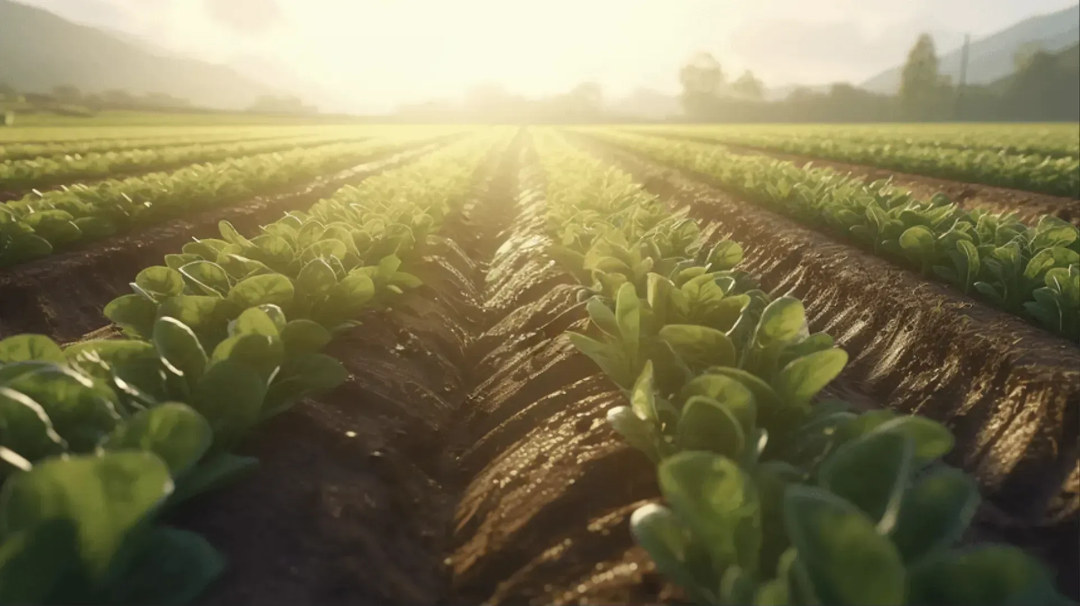
\includegraphics[width=0.8\textwidth,trim=0cm 5cm 0cm 0.2cm, clip]{./figures/intro.png}
	\caption{Forest-to-farm agricultural ecosystem.}
\end{figure}
	
\subsection{Restatement}
\hspace{1.5em}The primary goal of the modelling process is to track habitat change from forest-to-farm where diverse indicators ought to be considered, including human factors and natural processes, etc.
\begin{enumerate}
		\item Establish a food web model considering both natural and human factors, including food chain components, seasonal characteristics, chemical usages, etc. Their corresponding impacts on the ecosystem stability is required to be analyzed.
		\item Analyze the influence of native species' reemergence and their interactions with environments,  using two species as the case study.
		\item Consider the impacts on ecosystem stability when herbicide is removed. When bats are incorporated, describe how they interact with other creatures and identify a similar species. 
\end{enumerate}
	
	\section{Assumptions and Justifications}
\hspace{1.5em}\textbf{Assumption 1: }Total biomass and species quantity of living creatures in agricultural ecosystems follow a distribution strictly based on a certain proportion during specified periods, and the ecosystem being studied feature a finite geographical area.

\textbf{Justification 1: }Biomass and species richness of the given agricultural ecosystem are generally  influenced by factors including resource availability, human interventions and other climate-related elements, all of which operate within a predictable temporal and spatial framework. They constrain the evolution process of ecosystems, leading to a forseeable species distribution and biomass accumulation during specific periods. 

\textbf{Assumption 2: }In the primary stage of agricultural ecosystem evolution, biodiversity and species richness are positively proportional to ecosystem stability.

\textbf{Justification2: }Existing researches \cite{1} \cite{2} \cite{3} have revealed that either low or high phylogenetic diversity enhances stability directly.
	
	
\section{Notations}
	
	
\section{Sensitivity and Robustness Analysis}
\hspace{2em}\textbf{Sensitivity Analysis. }Since our EEDM model is a crucial part in the simulation of human impacts on agricultural ecosystems, we calculate the Sensitivity Coefficient for Equation \ref{primitive} and \ref{time}, which goes as:
\begin{equation}
	Sensitivity\ Coefficient(SC\  \text{for short})=\frac{\frac{\partial LSR}{\partial t}\times t}{LSR}=\frac{(-0.02924\times t+59.17)\times t}{-0.01462\times t^2+59.17\times t-59845.89}
\end{equation}
where $LSR$ stands for Losses of Species Richness effected by humans' overuse of chemicals and $t$ for year. Let $t=2025$, we have $SC=-2.851556$. From figure \ref{ti}, we have $LSR(t=2025)=27.6\%$ which indicates that $LSR$ will drop to $26.8129\%$ till year 2045. Therefore, the output quantity of EEDM isn't sensitive to time . Considering the practical meaning of EEDM model, such result implicates that if no measures are deliberately taken to reduce chemical use, our ecosystems may suffer severe losses in biodiversity at an astonishing rate and the deteriorating speed isn't likely to shrink automatically.

\textbf{Robustness Analysis. }The Monte Carlo Algorithm is employed to test the robustness of our MLP neural network proposed in section 4.2, the result is illustrated in figure \ref{mt}. 
\begin{figure}[h]
	\centering
	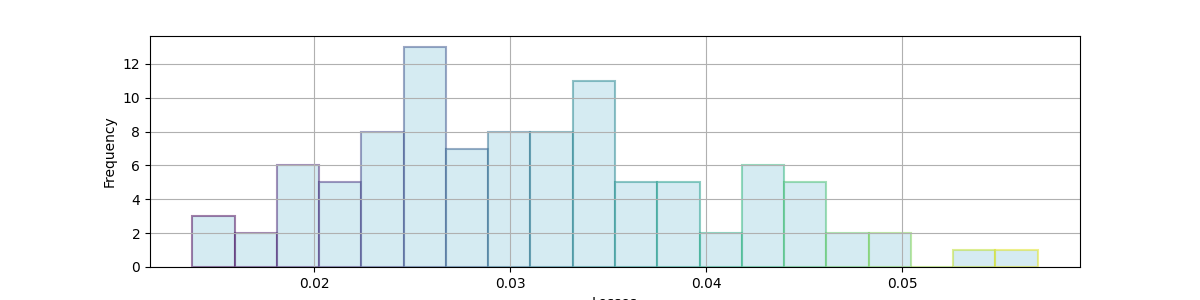
\includegraphics[width=\textwidth,trim=0cm 0.1cm 0cm 0.92cm,clip]{./figures/Monte Carlo.png}
	\caption{Results of Monte Carlo Robustness Testing.}
	\label{mt}
\end{figure}
	
From figure \ref{mt} we have $Mean\ loss=0.03123$, $Standard\ Deviation\ of\ Loss=0.00917$. Therefore we reach to the conclusion that our model converges successfully and features strong robustness and generalization ability, which as well proves the rationality of our following analysis.
	
	
	
	
	
	
	
	
	
	
	
	
	
	
	
	
	

	%%%%%%%%%% 正文结束 %%%%%%%%%%%%
	%%%%%%%%% 参考文献开始 %%%%%%%%%%%%
	\newpage
	\begin{thebibliography}{00}
\bibitem{1} 
Craven, D.; Eisenhauer, N.; Hautier, Y.; et al. Multiple facets of biodiversity drive the diversity-stability relationship [J]. \emph{Nature ecology\& evolution}, \textbf{2018}, \emph{2}, 1579--1587.
		
\bibitem{2}
Mougi, A. Ecosystem engineering and food web stability [J]. \emph{Scientific reports}, \textbf{2024}, \emph{14}, DOI: 10.1038/s41598-024-70626-w 
		
		
\bibitem{3} % 第二个参考文献
Hatton, I.A.; Mazzarisi, O.; Altieri, A.; Smerlak, M. Diversity begets stability: Sublinear growth and competitive coexistence across ecosystems [J]. \emph{Science}, \textbf{2024}, \emph{383}, DOI:10.1126/science.adg8488

\bibitem{标准氮肥用量和地区物种丰度间的关系}
Zhao, J.; Yu, L; Newbold, T.; etc. Biodiversity responses to agricultural practices in cropland and natural habitats [J]. \emph{Science of the Total Environment}, \textbf{2024}, \emph{922}, DOI:10.1016/j.scitotenv.2024.171296

\bibitem{攻击模型的所有数据}
https://ourworldindata.org


	\end{thebibliography}
	%%%%%%%%% 参考文献结束 %%%%%%%%%
	%%%%%%%%% 全文结束 %%%%%%%%%%%%%
\end{document}
\end
